\begin{lstlisting}
p58 1 2 3 7 8 9 10
\end{lstlisting}
\begin{exercise}
\begin{figure}[H]
\centering

\includegraphics[width=\textwidth]{1-hw5-2025032512.png}
% \caption{}
\label{}
\end{figure}
\end{exercise}
记
\[
\gamma_1:[0,1]\to l_{-i\to i}\qquad t\mapsto-i+2ti
\]
\[
\gamma_2:[0,1]\to C^{-}_{-i\to i}\qquad t\mapsto e^{ -\frac{\pi}{2}i-t\pi i }
\]
\[
\gamma_3:[0,1]\to C^{+}_{-i\to i}\qquad t\mapsto e^{ -\frac{\pi}{2}i+t\pi i }
\]
于是

(1)
\[
I_1=\int_{\gamma_1}^{} \lvert z \rvert  \, dz =\int_{0}^{1} \lvert -i+2ti \rvert 2i  \, dt=i
\]
(2)
\[
I_2=\int_{\gamma_2}^{} \lvert z \rvert  \, dz =\int_{0}^{1} \left\lvert  e^{ -\frac{\pi}{2}i-t\pi i }  \right\rvert e^{ -\frac{\pi}{2}i-t\pi i }\cdot (-\pi i)  \, dt=2i
\]
(3)
\[
I_3=\int_{\gamma_3}^{} \lvert z \rvert  \, dz =\int_{0}^{1} \left\lvert  e^{ -\frac{\pi}{2}i+t\pi i }  \right\rvert \pi i \cdot e^{ -\frac{\pi}{2}i+t\pi i } \, dt=2i
\]
\begin{exercise}
\begin{figure}[H]
\centering

\includegraphics[width=\textwidth]{2-hw5-2025032512.png}
% \caption{}
\label{}
\end{figure}
\end{exercise}
记
\[
\gamma_1:[0,1]\to C^{+}_{1\to1}\qquad t\mapsto e^{ 2\pi it }
\]
\[
\gamma_2:[0,1]\to l_{z_1\to z_2}\qquad t\mapsto z_1+t(z_2-z_1)
\]
(1)
\[
I_1=\int_{\gamma_1}^{} \mathrm{Re} z \, dz=\int_{0}^{1} \cos(2\pi i t) e^{ 2\pi i t  }2\pi i\, dt=\frac{1}{2} (-1+i \sinh (2 \pi )+\cosh (2 \pi ))
\]
(2)
\[
I_2=\int_{\gamma_2}^{} \mathrm{Re}z \, dz=\int_{0}^{1} \mathrm{Re}[z_1+t(z_2-z_1)]\cdot(z_2-z_1) \, dt =\frac{1}{2}(\mathrm{Re}z_2-\mathrm{Re}z_1)(z_2-z_1)
\]
\begin{exercise}
\begin{figure}[H]
\centering
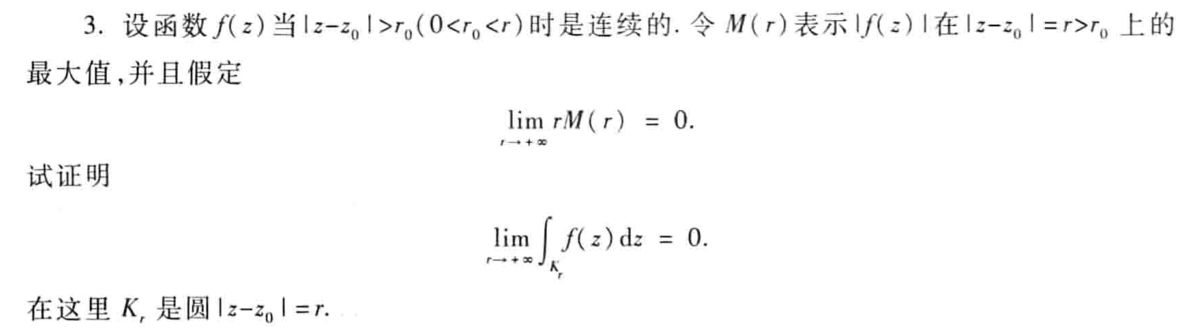
\includegraphics[width=\textwidth]{3-hw5-2025032512.png}
% \caption{}
\label{}
\end{figure}
\end{exercise}
\begin{proof}
当 $r>r_0$ 时,
\[
\left\lvert  \int_{K_{r}}^{} f(z) \, dz  \right\rvert \leq \int_{K_{r}}^{} M(r) \, dz =2\pi r \cdot M(r)
\]
令 $r \to \infty$ 得到
\[
\lim_{ r \to \infty } \int_{K_{r}}^{} f(z) \, dx =0
\]
\end{proof}

\begin{exercise}
\begin{figure}[H]
\centering

\includegraphics[width=\textwidth]{hw5-2025032720.png}
% \caption{}
\label{}
\end{figure}
\begin{figure}[H]
\centering

\includegraphics[width=\textwidth]{1-hw5-2025032720.png}
% \caption{}
\label{}
\end{figure}
\end{exercise}
(1)
$\sqrt{ z }=\sqrt{ \lvert z \rvert }\cdot e^{ \frac{i}{2}\arg z }$,
\[
I=\int_{C}^{} \frac{1}{\sqrt{ \lvert z \rvert  }} e^{ -\frac{i}{2}\arg z } \, dz=\int_{0}^{2\pi} e^{ -\frac{i}{2}\theta }\cdot ie^{ i\theta } \, d\theta=\int_{0}^{2\pi} i\cdot e^{ \frac{i}{2}\theta } \, d\theta =  -4
\]
$\sqrt{ z }=\sqrt{ \lvert z \rvert }e^{ \frac{i}{2}\arg z }$,
\[
I=\int_{C}^{} \frac{1}{\sqrt{ \lvert z \rvert  }} e^{ -\frac{i}{2}\arg z } \, dz=4
\]
(2)
$\ln z=\ln \lvert z \rvert+i\arg z$,
\[
\begin{aligned}
I & =\int_{0}^{2\pi} (\ln \lvert e^{ i\theta } \rvert+i\theta) ie^{ i\theta } \, d\theta=\int_{0}^{2\pi} -\theta e^{ i\theta } \, d\theta \\
 & =\int_{0}^{2\pi} i\theta \, de^{ i\theta }=\left.(i\theta e^{ i\theta })\right| ^{2\pi}_{0}-\int_{0}^{2\pi} e^{ i\theta  } \, d(i\theta) \\
 & =2\pi i
\end{aligned} 
\]
$\ln z=\ln \lvert z \rvert+i\arg z+2\pi i$,
\[
\begin{aligned}
I & =\int_{0}^{2\pi} (\ln \lvert e^{ i\theta } \rvert +i\theta+2\pi i)\cdot ie^{ i\theta } \, d\theta  \\
 & =\int_{0}^{2\pi} -(2\pi+\theta)\cdot e^{ i\theta } \, d\theta \\
  & =-\int_{0}^{2\pi} \theta e^{ i\theta } \, d\theta \\
  & =2\pi i
\end{aligned}
\]
\begin{exercise}
\begin{figure}[H]
\centering
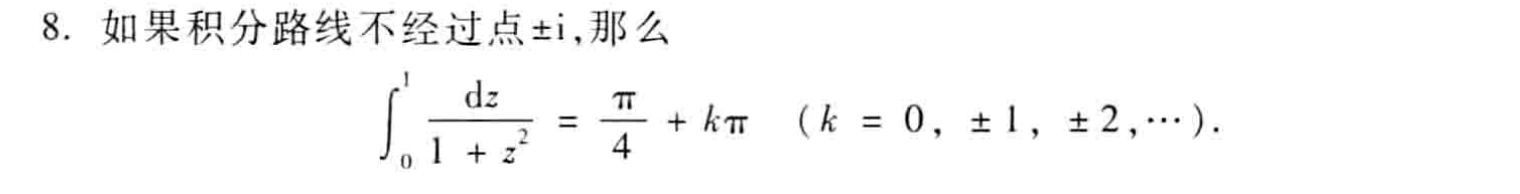
\includegraphics[width=\textwidth]{2-hw5-2025032720.png}
% \caption{}
\label{}
\end{figure}
\end{exercise}
Let
\[
\gamma_0:[0,1]\to[0,1]\qquad t\mapsto t
\]
Then
\[
\int_{\gamma_0}^{} \frac{1}{1+z^2}  \, dz=\int_{0}^{1} \frac{1}{1+x^2}  \, dx =\frac{\pi}{4}
\]
$f (z)\coloneqq \frac{1}{1+z^2}$ is holomorphic in $\mathbb{C}\setminus \{ \pm i \}$, then for any
\[
\gamma:[0,1]\to C_{0\to1}
\]
with $\mathrm{Ind}_{i}(\gamma)=n,\mathrm{Ind}_{-i}(\gamma)=m$. We have
\[
\int_{\gamma}^{} f(z) \, dz +\int_{\gamma_0^{-}}^{} f(z) \, dz +n\int_{C_{i}(\epsilon)}^{} f(z) \, dz+m\int_{C_{-i}(\epsilon)}^{} f(z) \, dz  =0
\]
where
\[
\begin{aligned}
\int_{C_i(\epsilon)}^{} f(z) \, dz & =\int_{C_i(\epsilon)}^{} \frac{1}{1+z^2}  \, dz=\frac{1}{2i} \int_{C_i(\epsilon)}^{} \left( \frac{1}{z-i} -\frac{1}{z+i} \right) \, dz \\
 & =\frac{1}{2i }\underbrace{ \int_{C_i(\epsilon)}^{} \frac{1}{z-i}  \, dz }_{ =2\pi i }-\frac{1}{2i} \underbrace{ \int_{C_i(\epsilon)}^{} \frac{1}{z+i}  \, dz }_{ =0 }    \\
 & =\pi
\end{aligned}
\]
Similarly,
\[
\int_{C_{-i}(\epsilon)}^{} f(z) \, dz =-\pi
\]
Therefore
\[
\int_{\gamma}^{} f(z) \, dx -\frac{\pi}{4}+(n-m)\pi=0
\]
\[
\int_{\gamma}^{} \frac{1}{1+z^2}  \, dz=\frac{\pi}{4}+k\pi \qquad k=0,\pm1,\pm2,\dots
\]
where $k=m-n=\mathrm{Ind}_{i}(\gamma)-\mathrm{Ind}_{-i}(\gamma)$.

\begin{figure}[H]
\centering
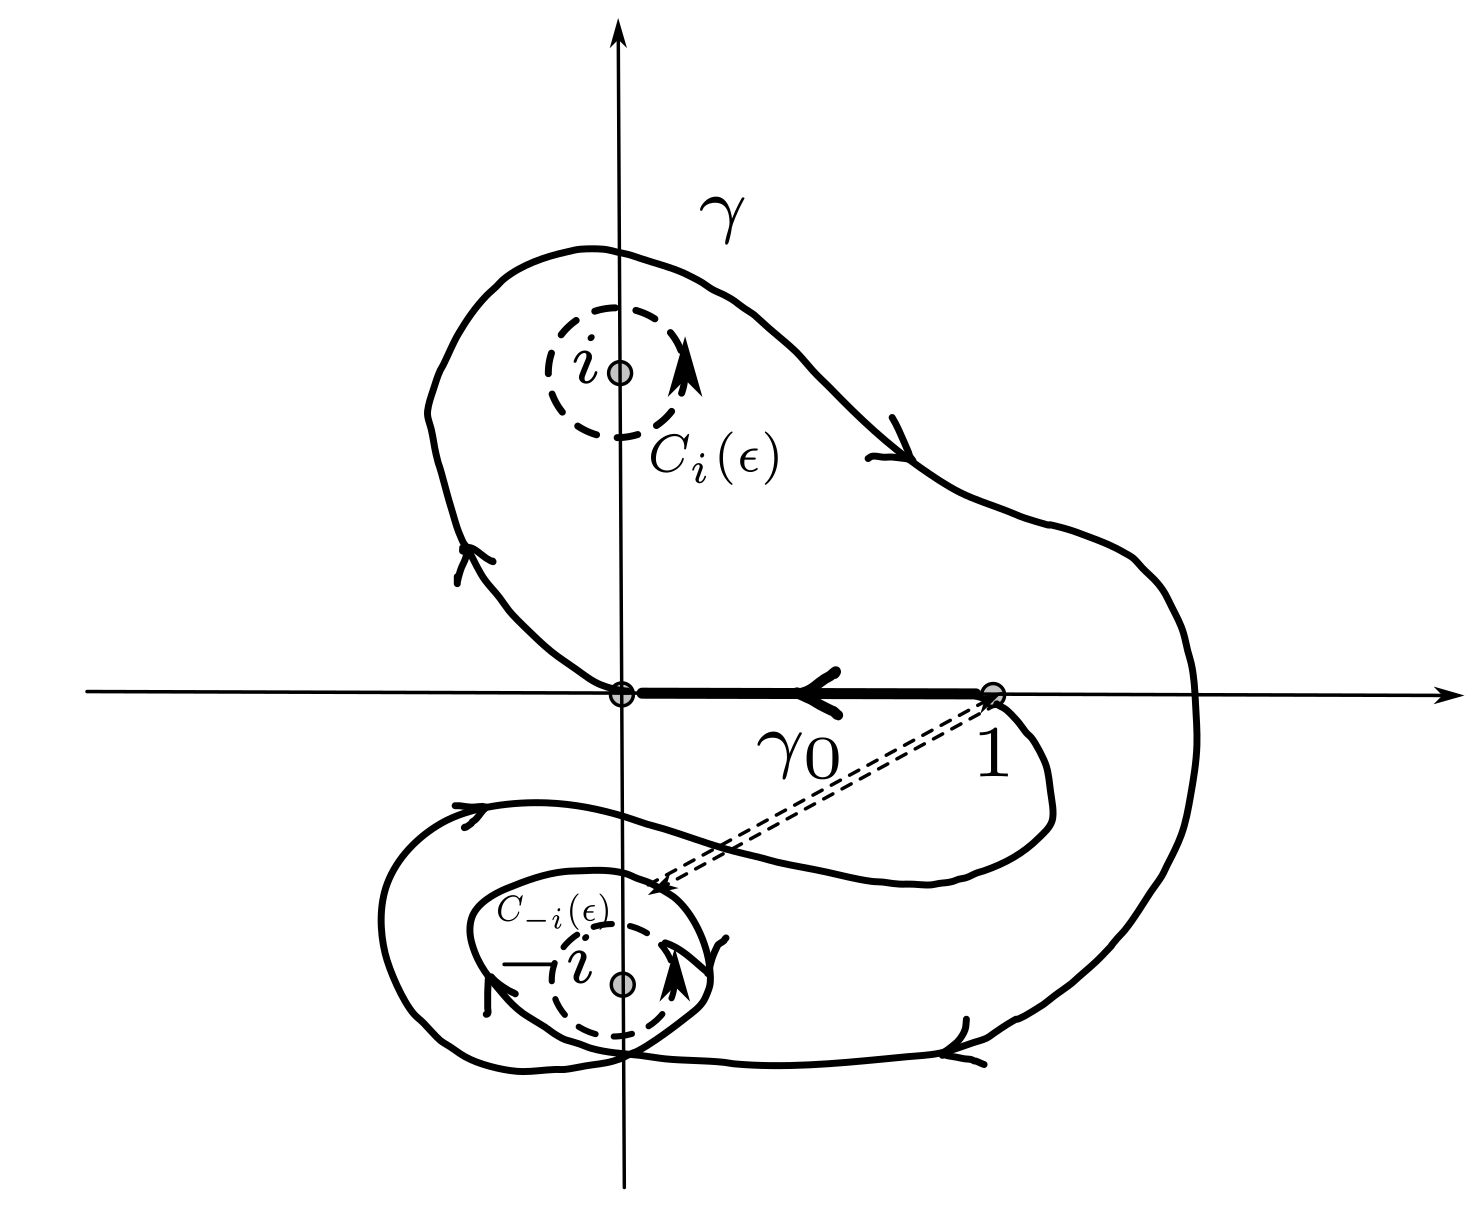
\includegraphics[width=\textwidth]{2-hw5-2025032721.png}
% \caption{}
\label{}
\end{figure}

\begin{exercise}
\begin{figure}[H]
\centering
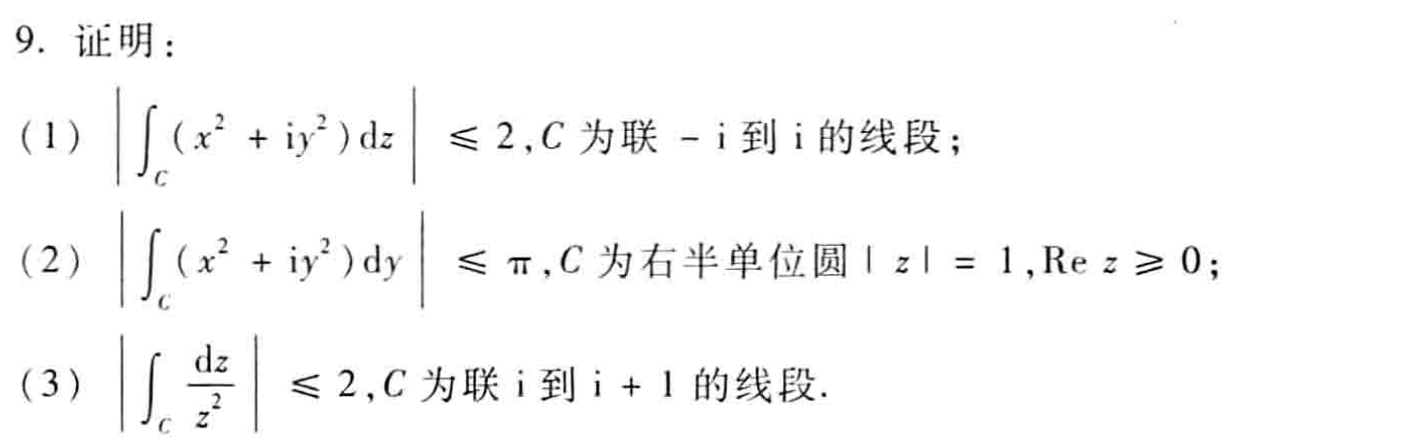
\includegraphics[width=\textwidth]{3-hw5-2025032720.png}
% \caption{}
\label{}
\end{figure}
\end{exercise}
(1)
\[
C:[0,1]\to l_{-i\to i}\qquad t\mapsto-i+2ti
\]
\[
\left\lvert  \int_{C}^{} (x^2+iy^2) \, dz   \right\rvert=\left\lvert  \int_{0}^{1} i(2t-1)^2(-1)(2i) \, dt   \right\rvert =\left\lvert  \int_{0}^{1} 8t^2-8t+2 \, dt  \right\rvert =\frac{2}{3}\leq 2
\]
(2)
\[
\begin{aligned}
\lvert I \rvert  & \leq \int_{\lvert z \rvert =1,\mathrm{Re}z\geq 0}^{} \lvert x^2+iy^2 \rvert  \, dy =\int_{\lvert z \rvert =1,\mathrm{Re}z\geq 0}^{} \sqrt{ x^{4}+y^{4} } \, dy \\
 & \leq \int_{\lvert z \rvert =1,\mathrm{Re}z\geq 0}^{} \underbrace{ (x^2+y^2)^2 }_{ =1 } \, dy\leq \int_{\lvert z \rvert =1,\mathrm{Re}z\geq 0}^{}  \, dz=\pi
\end{aligned}
\]
(3)
\[
\lvert I \rvert \leq \int_{l_{i\to i+1}}^{} \underbrace{ \frac{1}{\lvert z \rvert ^2} }_{ \leq 1/(1/\sqrt{ 2 })^2 }   \, dz \leq \int_{l_{i\to i+1}}^{} 2 \, dz=2
\]
\begin{exercise}
\begin{figure}[H]
\centering
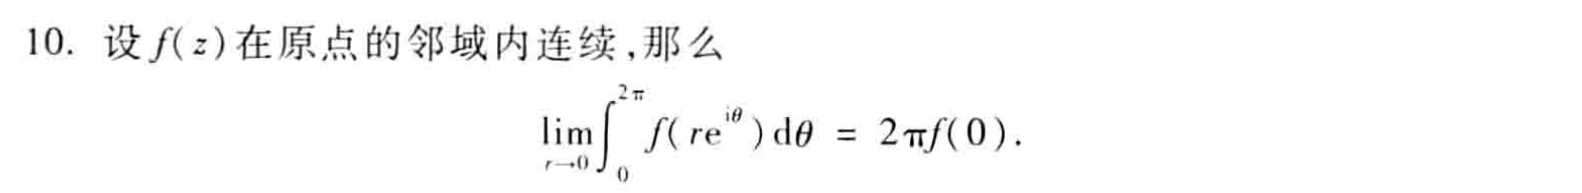
\includegraphics[width=\textwidth]{4-hw5-2025032720.png}
% \caption{}
\label{}
\end{figure}
\end{exercise}
Since $f$ is continuous in the neighborhood of 0, then for any $\epsilon>0$, there exists $\delta>0$, s.t.
\[
\lvert f(z)-f(0) \rvert <\epsilon,\qquad \forall \lvert z \rvert <\delta
\]
Let $r<\delta$, then
\[
\left\lvert  \int_{0}^{2\pi} f(re^{ i\theta })-f(0)  \, d\theta  \right\rvert\leq \int_{0}^{2\pi} \underbrace{ \lvert f(re^{ i\theta })-f(0) \rvert }_{ \leq \epsilon }  \, d\theta\leq 2\pi\epsilon 
\]
Since $r$ can be arbitrarily small, thus we have
\[
\lim_{ r \to 0 } \int_{0}^{2\pi} f(re^{ i\theta }) \, d\theta=2\pi f(0)
\]